\chapter{Pornirea sistemului}
\label{chapter:boot}

Atunci când un sistem hardware pornește, acesta urmărește încărcarea sistemului
de operare, pornirea acestuia și a proceselor de bază. Această se acțiune se
cheamă \textit{booting} sau \textit{bootstrapping}: modul în care un sistem, din momentul în care
este alimentat și pornit fizic, ajunge să ofere o interfață de lucru
utilizatorului. Procesul de boot/booting se referă la pașii urmați de la
pornirea electrică (\textit{power on}) până la pornirea proceselor.

Înțelegerea procesului de boot este utilă pentru un utilizator dacă dorește să
își configureze modul în care este configurat hardware-ul sistemului, ce sistem
de operare rulează, opțiuni de rulare a sistemului de operare și ce procese sunt
create la pornire (\textit{startup}). Pentru un utilizator avizat, a ști informații
despre anatomia procesului de boot și a secvența de pași urmați este important
pentru a depana probleme ce pot apărea sau pentru a îmbunătăți aspecte precum
timpul de pornire, securitatea sistemului, consumul de resurse.

După pornirea fizică
(power on) a sistemului, este încărcat firmware-ul de boot (numit BIOS pe
arhitectura x86), apoi este identificat un dispozitiv bootabil, este încărcat
bootloaderul, apoi sistemul de operare și apoi sunt pornite procesele de
început (\textit{startup processes}). În \labelindexref{Figura}{fig:boot:sequence} este prezentat un sumar al
pașilor urmați în secvența de boot, urmând să îi detaliem în secțiunile de mai
jos:

\begin{figure}[htbp]
	\centering
	\def\svgwidth{0.5\columnwidth}
	\includesvg{chapters/09-boot/img/boot-seq.svg}
        \caption{Secvența de boot pe PC}
	\label{fig:boot:sequence}
\end{figure}

\begin{enumerate}
	\item firmware de boot (BIOS)
	\item dispozitiv bootabil
	\item bootloader
	\item sistem de operare (kernel) și drivere de dispozitiv
	\item procese inițiale
\end{enumerate}

\section{Secvența de boot}
\label{sec:boot:sequence}

În cadrul secvenței de boot, fiecare pas, descris în
\labelindexref{Figura}{fig:boot:sequence}, are rolul său. Unul dintre
roluri este acela de a transfera controlul următorului pas: fiecare pas are
capacitate limitată în procesul de pornire, următorul pas preluând rezultatul
său și realizând alte acțiuni. Alt rol al fiecărui pas este de configurare a
unor opțiuni specifice în procesul de boot, așa cum vom preciza mai jos.

În momentul pornirii fizice (\textit{power on}), sistemul încarcă firmware-ul de boot dintr-o zonă
dedicată. Firmware-ul de boot este
numit BIOS (sau UEFI \abbrev{UEFI}{Unified Extensible Firmware Interface}) pe
arhitectura x86. Firmware-ul de boot există pe sistemul fizic indiferent de
prezența sau nu a unui sistem de operare sau dispozitiv bootabil. Firmware-ul de
boot realizează verificări de bază ale funcționării hardware-ului, oferă
utilizatorului posibilitatea de configurări aproape de hardware (precum
activarea/dezactivarea virtualizării, configurarea vitezei de acces la memorie)
și stabilește ordinea de boot: ce dispozitive și în ce ordine sunt verificate
pentru a trece la următorul pas.

Firmware-ul de boot identifică dispozitivul de boot și încarcă o secvență
dedicată de pe acesta. Dispozitivul de boot poate fi hard disk drive, USB flash
drive, CD-ROM drive. Dispozitivul de boot nu are un rol activ, ci unul de
stocare. Acesta stochează următoarea secvență de cod care să fie executată, în
mod tipic bootloaderul. Bootloaderul este încărcat de firmware-ul de
boot din dispozitivul de boot în memorie. Apoi îi este transferat controlul
bootloaderului.

Întrucât firmware-ul de boot are, de obicei, capacități limitate de a încărca în
memorie părți stocate pe un dispozitiv precum hard disk, se transferă controlul
bootloaderului pentru a gestiona acest lucru. Bootloaderul urmărește
încărcarea în memorie a sistemului de operare (a imaginii de kernel) de pe un dispozitiv de stocare.
Bootloaderul poate oferi opțiunea
utilizatorului de a decide ce sistem de operare să încarce, funcționalitate
utilă pentru sistemele dual boot (când putem boota și Windows și Linux).

Sistemul de operare este pornit cu ajutorul bootloaderului din imaginea de
kernel. Imaginea de kernel este un fișier care se regăsește pe un dispozitiv de
stocare; din acest dispozitiv este încărcată în memorie și îi este transferat controlul.
Imaginea de kernel este practic un fișier executabil care conține datele și
codul sistemului de operare. Transferul controlului înseamnă execuția codului
sistemului de operare. Din acest punct, sistemul de operare deține controlul
sistemului și asigură buna funcționare a acestuia.

O dată încărcat sistemul de operare, acesta încarcă și driverele de dispozitiv
(\textit{device drivers}). Driverele de dispozitiv sunt reținute în fișiere similare
imaginii de kernel și sunt încărcate în memorie de către sistemul de operare
pentru gestionarea dispozitivelor hardware: disc, rețea, tastatură etc.

După încărcarea driverelor, sistemul de operare pornește primele procese ale
sistemului (\textit{startup processes}). Aceste procese sunt serviciile de bază ale
sistemului (precum menținerea timpului sistemului, aplicarea configurațiilor de
rețea) și aplicațiile de interfață cu utilizatorul (shellurile). Acum
utilizatorul se poate autentifica în sistemul de operare și poate beneficia de
serviciile acestuia.

Secvența de pași de bootare este comună pentru arhitecturi hardware și sisteme
de operare diferite, dar fiecare pas are caracteristici și denumiri particulare.
Pe arhitectura x86 firmware-ul de boot se numește BIOS sau UEFI; pe arhitectura
ARM nu are o denumire specifică. Bootloaderele cele mai comune folosite pe arhitectura x86 sunt
GRUB (pentru Linux) sau WinLoader (pentru Windows), în vreme ce Das U-boot e un
bootloader folosit pentru platforme embedded precum ARM.

În cele ce urmează vom descrie în detaliu pașii din secvența de boot.

\section{Firmware de boot}
\label{sec:boot:firmware}

Firmware-ul de boot este o secvență de cod localizată pe un chip specific al
sistemului, în general un chip ROM (\textit{read-only memory}). Din acest motiv i se mai
spune și \textbf{boot ROM}. Firmware-ul de boot are următoarele roluri:

\begin{itemize}
	\item inițializează și verifică componentele hardware ale sistemului
	\item permite configurarea componentelor și opțiunilor hardware ale
		sistemului
	\item parcurge lista cu dispozitive de stocare posibile pentru a
		transfera controlul către unul dintre acestea
\end{itemize}

Firmware-ul de boot este rulat în momentul pornirii sistemului (adică la
apăsarea pe butonul de pornire). Este prima secvență de cod executată de
sistemul de calcul. Partea de verificare a componentelor hardware poartă numele
de POST \abbrev{POST}{Power-On Self Test} (\textit{Power-On Self Test}) pe arhitectura
x86; dacă sunt defecte hardware acestea vor fi semnalizate de firmware-ul de
boot, în general prin mesaje sonore sau vizuale simple.

Firmware-ul de boot este parte a hardware-ului sistemului și vine ,,preinstalat''
pe un chip al acestuia. În mod obișnuit, firmware-ul de boot este furnizat de
producătorul plăcii de bază care conține și acel chip.

Firmware-ul de boot permite realizarea de configurări la nivelul sistemului și
hardware-ului. Mai jos sunt o serie de configurări permise de firmware-ul de
boot:

\begin{itemize}
	\item stabilirea unei parole de protejare a meniului de configurare
	\item configurarea timpul sistemului
	\item activarea suportului hardware de virtualizare
	\item stabilirea viteză de acces la memorie
	\item activarea bootării de pe stick USB
	\item configurarea ordinii de boot
	\item activarea/dezactivarea folosirii porturilor USB
\end{itemize}

\subsection{BIOS și UEFI}
\label{sec:boot:firmware:bios-uefi}

Pe arhitectura x86, firmware-ul de boot poartă numele de BIOS (\textit{Basic
Input-Output System}). În ultima perioadă, BIOS este înlocuit de UEFI
(\textit{Unified Extensible Firmware Interface}). UEFI este o formă îmbunătățită de
firmware de boot, ușor de observat prin faptul că oferă o interfața grafică mai prietenoasă pentru configurare (de obicei se
folosește mouse-ul). Un avantaj al UEFI este dezvoltarea într-o formă
standardizată de un consorțiu din care fac parte producători de software și
hardware, ceea ce duce la caracteristici comune indiferent de sistemul hardware
folosit. \labelindexref{Figura}{fig:boot:bios-uefi} conține screenshoturi cu un ecran de boot BIOS\footnote{\url{https://commons.wikimedia.org/wiki/File:Bios-configuracion-smart-habilitada.png} (CC BY-SA 3.0)} și unul de boot
UEFI\footnote{\url{https://commons.wikimedia.org/wiki/File:Bios\_asus.jpg} (CC BY-SA 4.0)}.

\begin{figure}[!htbp]
  \centering
  \begin{subfigure}[b]{0.8\textwidth}
    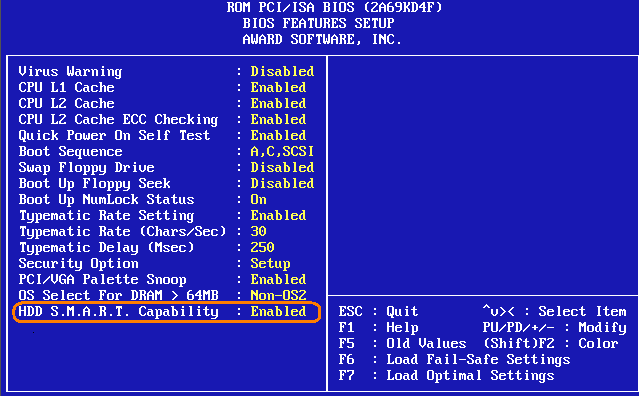
\includegraphics[width=\textwidth]{chapters/09-boot/img/bios.png}
    \caption{BIOS}
    \label{fig:intro:bios}
  \end{subfigure}

  \begin{subfigure}[b]{0.8\textwidth}
    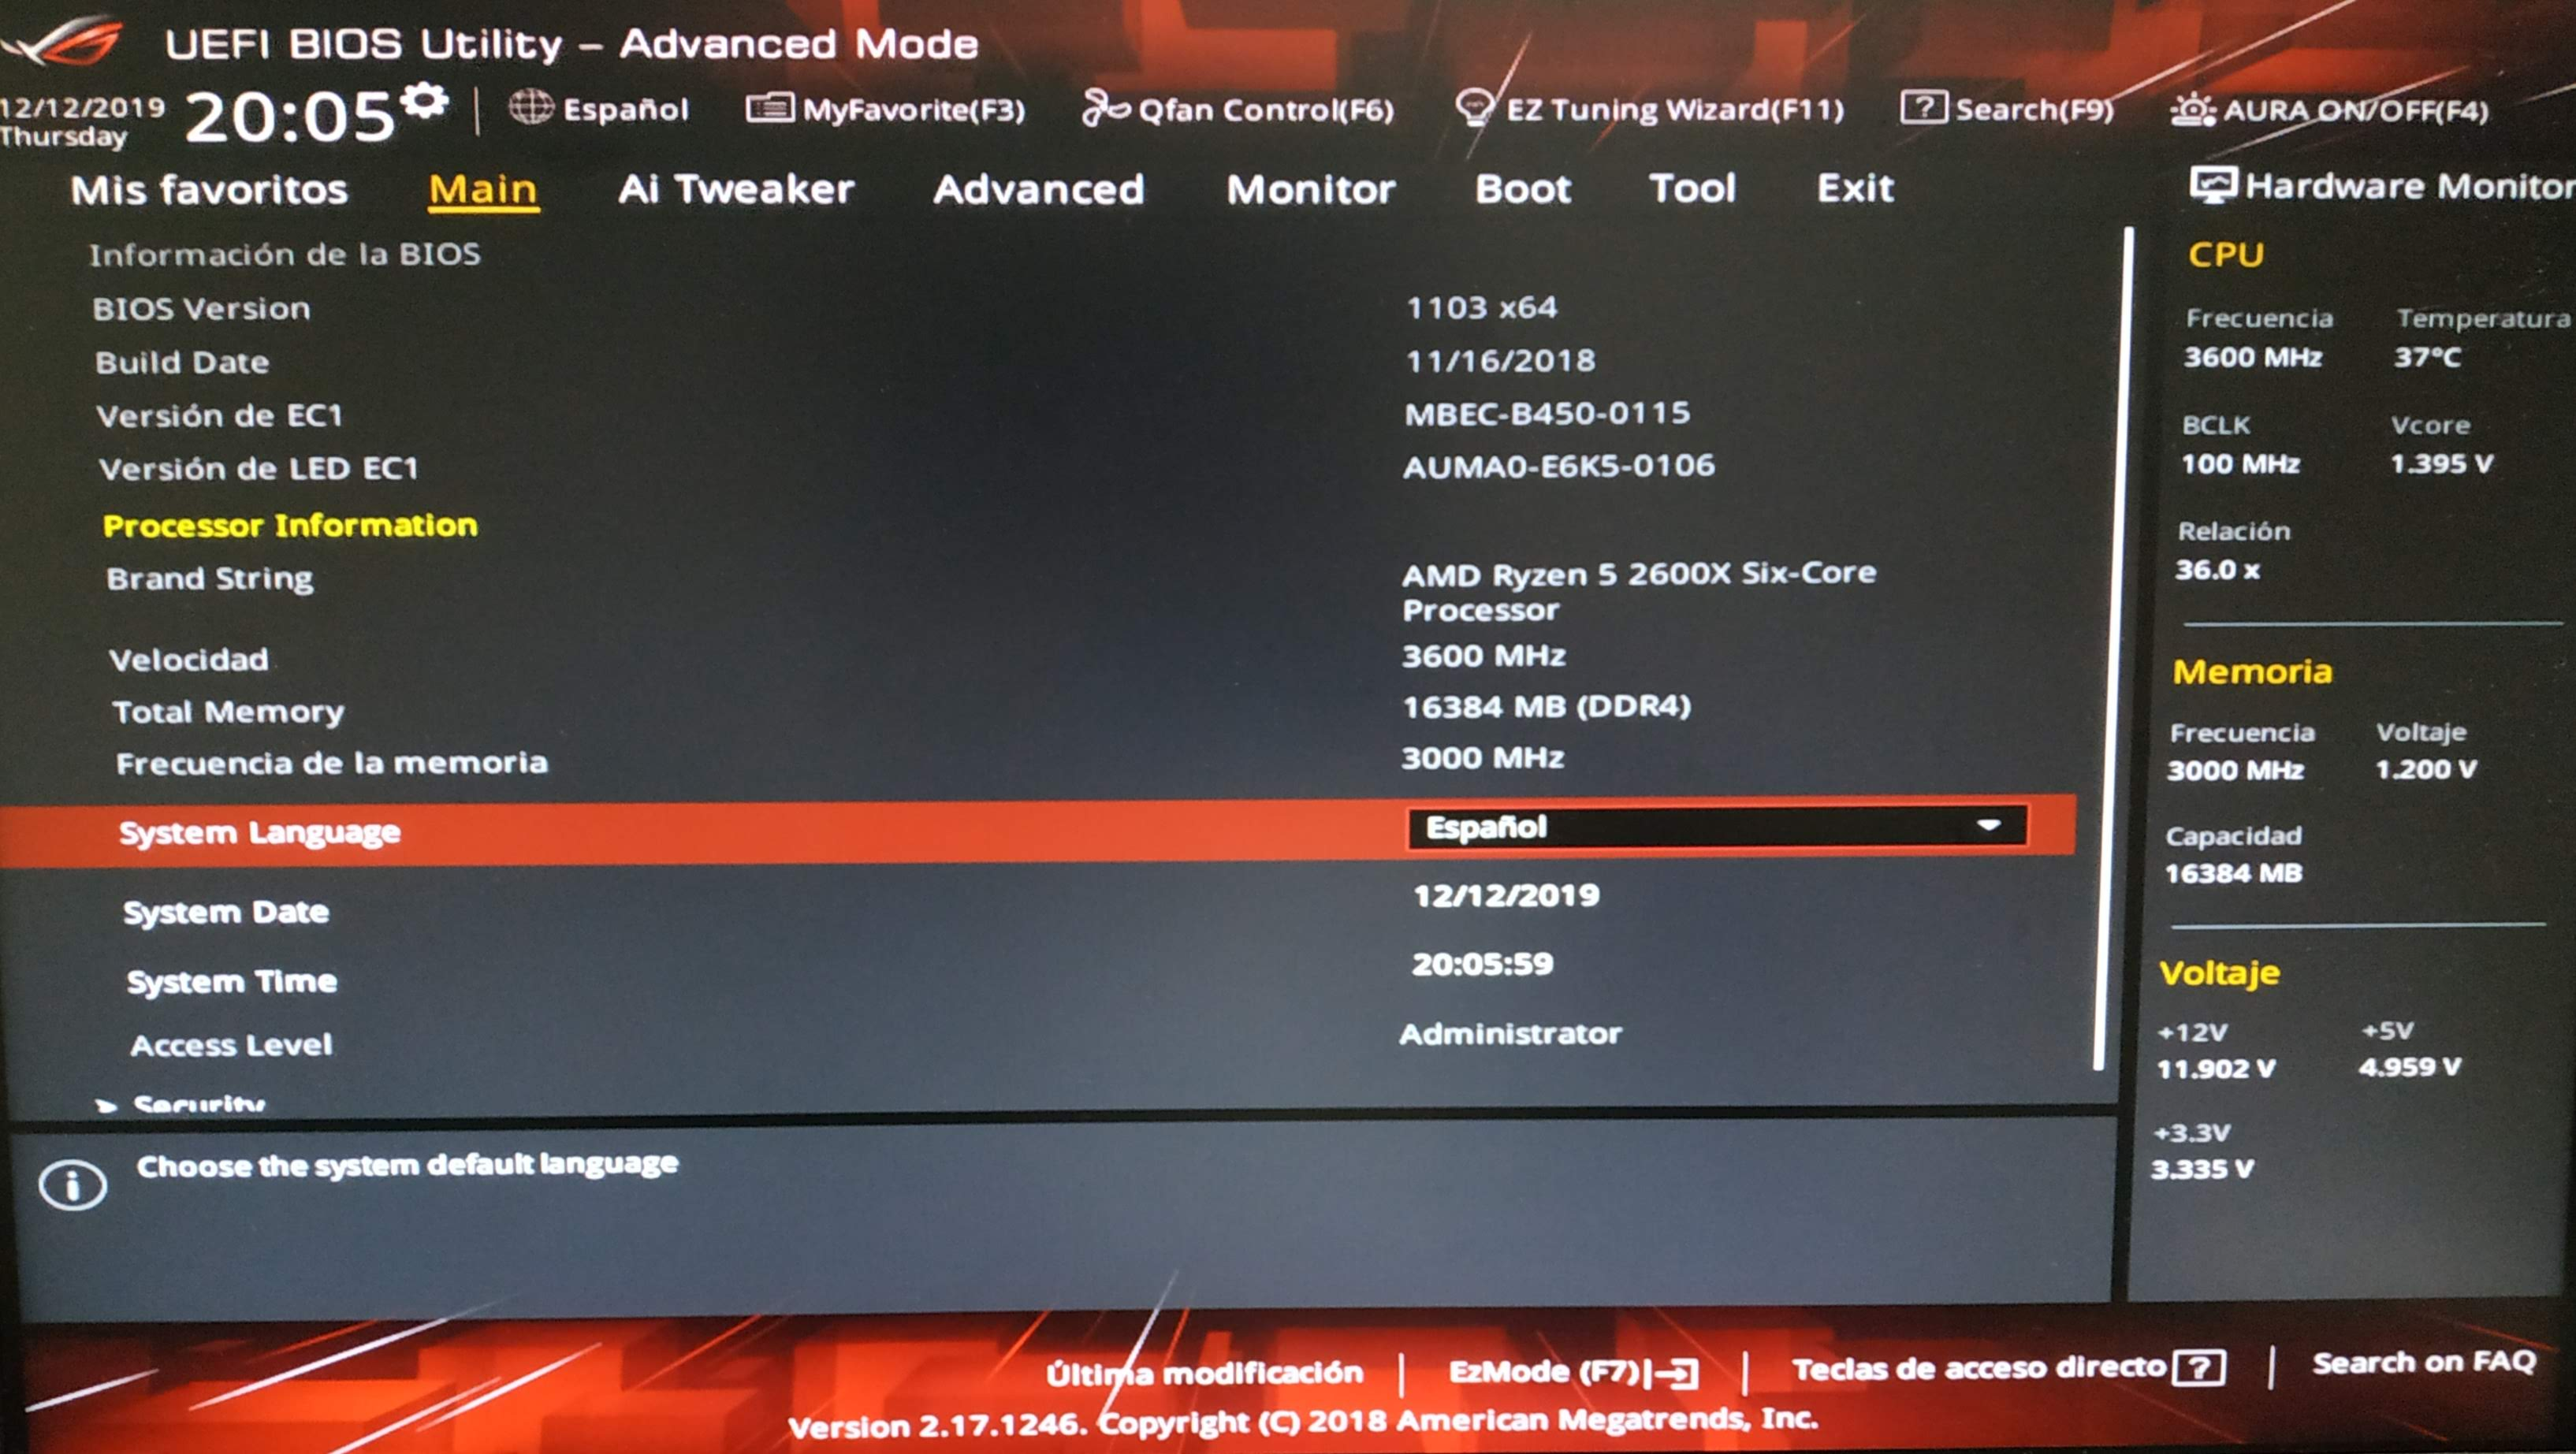
\includegraphics[width=\textwidth]{chapters/09-boot/img/uefi.jpg}
    \caption{UEFI}
    \label{fig:boot:uefi}
  \end{subfigure}
  \caption{BIOS și UEFI}
  \label{fig:boot:bios-uefi}
\end{figure}

Meniurile de configurare pentru BIOS și UEFI sunt accesate la pornirea sistemului
folosind o combinație de taste a furnizorului plăcii de bază, cel mai adesea \texttt{F2}, \texttt{F8}, \texttt{F12}
sau \texttt{Esc}. La apăsarea combinației adecvate se accesează ecranul de configurare
specific.

Configurațiile realizate sunt în mod uzual salvate la părăsirea modului de
configurare. Aceste configurații sunt salvate într-un chip de memorie dedicat
numit CMOS \abbrev{CMOS}{Complementary Metal-Oxide-Semiconductor} (de la
\textit{Complementary Metal-Oxide-Semiconductor}, tehnologia folosită pentru
tranzistoarele ce compun circuitele integrate moderne). Această memorie este
nevolatilă și își păstrează informațiile după resetarea sistemului. Chipul de
memorie este alimentat de o baterie dedicată numită baterie CMOS, similară cu
cea din \labelindexref{Figura}{fig:boot:cmos-battery}\footnote{\url{https://commons.wikimedia.org/wiki/File:Yakumo\_Notebook\_536S\_-\_CR2032\_backup\_battery\_on\_motherboard-4667.jpg} (\textcopyright{} Raimond Spekking / CC BY-SA 4.0 (via Wikimedia Commons))}.

\begin{figure}[!htbp]
  \centering
  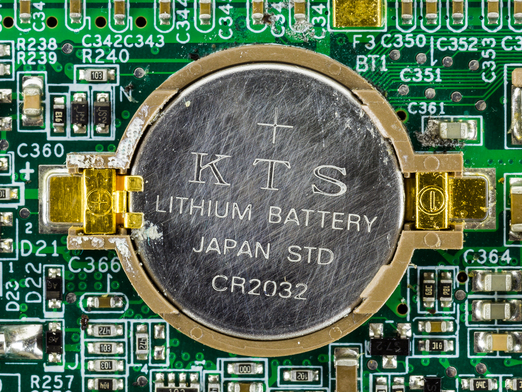
\includegraphics[width=0.8\textwidth]{chapters/09-boot/img/cmos-battery.jpg}
  \caption{Bateria CMOS}
  \label{fig:boot:cmos-battery}
\end{figure}

Dacă bateria CMOS este scoasă din soclul ei sau este epuizată, configurația se
pierd și BIOS-ul bootează la niște valori implicite. Aceasta este o formă facilă
de resetarea a parolei de BIOS, în cazul în care o astfel de parolă este
configurată, așa cum vom preciza în \labelindexref{Secțiunea}{sec:boot:pass-reset}.

Pe lângă interfața grafică mai prietenoasă, UEFI folosește o nouă schemă de
partiționare a discurilor numită GPT \abbrev{GPT}{GUID Partition Table} (\textit{GUID
Partition Table}) spre deosebire de schema MBR \abbrev{MBR}{Master Boot Record}
(\textit{Master Boot Record}) utilizată de BIOS. Aceasta îi permite o flexibilitate
sporită în accesarea dispozitivului de boot și alegerea următoarei faze din
procesul de boot: încărcarea bootloaderului. Vom reveni la schemele de partiționare GUID și MBR în \labelindexref{Secțiunea}{sec:boot:bootdev:scheme}; detalii vom prezenta și în \labelindexref{Secțiunea}{sec:storage:partition}.

În general, UEFI permite și un mod de booting compatibil cu BIOS. În acest mod,
procesul de bootare este similar cu cel de BIOS și se folosește tot schema de
partiționare MBR și modul de încărcare a bootloaderului. Altfel se folosește
modul nativ de bootare UEFI. UEFI folosește o partiție dedicată numită ESP (\textit{EFI
System Partition}), formatată cu sistem de fișiere FAT, în care stochează imagini
de firmware (numite imagini EFI) care rețin codul bootloaderului ce va fi
încărcat la următorul pas.

\labelindexref{Tabelul}{tab:boot:bios-uefi} prezintă principalele deosebiri\footnote{\url{https://www.freecodecamp.org/news/uefi-vs-bios/}} între BIOS și UEFI:

\begin{table}[!htb]
  \caption{Comparație BIOS-UEFI}
  \begin{center}
    \begin{tabular}{ p{0.40\textwidth} p{0.25\textwidth} p{0.25\textwidth} }
      \toprule
        \textbf{Criteriu} &
        \textbf{BIOS} &
        \textbf{UEFI} \\
      \midrule
        localizarea codului &
        chip EPROM pe placa de bază &
        fișiere \texttt{.efi} în partiția ESP \\

        schemă de partiționare implicită &
        MBR &
        GUID \\

        dimensiunea maximă a discului &
        2.2 TB &
        9 ZB \\

        ecran de configurare &
        text &
        grafic \\

        suport SecureBoot &
        nu &
        da \\

      \bottomrule
    \end{tabular}
    \label{tab:boot:bios-uefi}
  \end{center}
\end{table}

Datorită flexibilității, sistemele PC \abbrev{PC}{Personal Computer} moderne
folosesc din ce în ce mai mult UEFI, cu probabilitate mică de a mai întâlni, în următorii ani,
sisteme care folosesc BIOS. BIOS rămâne însă folosit pe
sistemele mai vechi și înțelegerea modului său de funcționare e utilă pentru a
vedea evoluția firmware-ului de boot pe arhitectura x86.

\subsection{Alte firmware-uri de boot}
\label{sec:boot:other}

Fiecare sistem hardware care rulează un sistem de operare generalist (\textit{general
purpose}) are un firmware de boot, prima componentă rulată la pornirea
sistemului. Pe arhitectura x86, de fapt pe sistemele de tipul PC (Personal
Computer), acest firmware de boot este BIOS-ul, iar în ultimii ani UEFI.

Sistemele care folosesc procesoare ARM sunt mai variate, fără să aibă un format
unitar de conectare a componentelor hardware. Mai mult, producătorii de sisteme
care folosesc arhitecturi ARM sunt foarte variați. Din acest motiv nu există un
standard universal precum BIOS sau UEFI pe ARM, lucru care face mai dificilă
dezvoltarea de software de sistem pentru o plajă de dispozitive ARM.

Pe sistemele PC o alternativă de firmware de boot este coreboot (și alternativa
libreboot). coreboot este o versiune liberă/deschisă de firmware de boot, ca o
reacție la faptul că firmware-ul de BIOS și UEFI este în general furnizată de producător în
formă binară (\textit{binary blob}). Dincolo de aspecte de filozofie (software liber vs.
proprietar), dezvoltatorii coreboot invocă posibilitatea ca furnizorii de binare
BIOS/UEFI să aibă accese ascunse (\textit{backdoor}), iar un firmware de boot deschis
oferă posibilitatea verificării codului. coreboot încă folosește unele
componente binare în vreme ce libreboot le înlocuiește pentru o versiune complet
deschisă. Dezavantajul coreboot este folosirea sa redusă pe sisteme hardware,
doar câteva folosind coreboot în loc de UEFI (sau BIOS).

\subsection{Configurare dispozitive bootabile}
\label{sec:boot:device-config}

Unul dintre rolurile firmware-ului de boot este configurarea dispozitivelor
bootabile și selectarea ordinii de boot. \labelindexref{Figura}{fig:boot:bios-boot-order}\footnote{\url{https://commons.wikimedia.org/wiki/File:Bios-configuracion-orden-arranque.png} (CC BY-SA 3.0)} afișează ecranul BIOS
pentru stabilirea ordinii dispozitivelor bootabile.

\begin{figure}[!htbp]
  \centering
  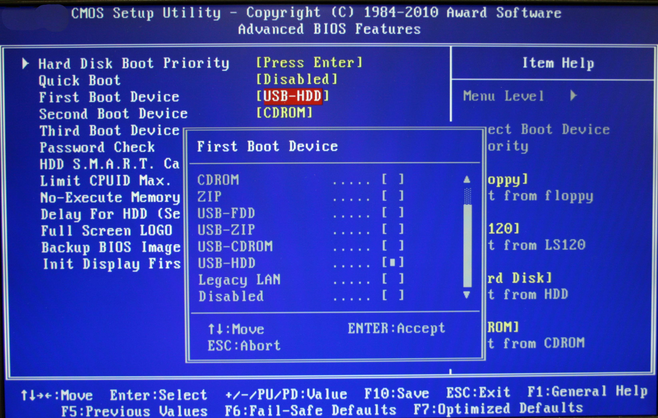
\includegraphics[width=0.8\textwidth]{chapters/09-boot/img/bios-boot-order.png}
  \caption{Stabilirea ordinii dispozitivelor bootabile în BIOS}
  \label{fig:boot:bios-boot-order}
\end{figure}

Atunci când firmware-ul va trece la pasul următor va trece, în ordine, prin
dispozitivele de boot configurate și va boota de pe primul disponibil.
Dispozitive de boot pot fi discuri, USB flash drive-url, CD ROM-drive sau poate fi vorba de
bootare din rețea folosind PXE \abbrev{PXE}{Preboot eXecution Environment}
(\textit{Preboot eXecution Environment}).

Un dispozitiv bootabil, identificat
ca atare de firmware, are un marcaj specific: conține o secvență de cod care este rulată de firmware și
care este următoarea fază a procesului de boot. Această secvență este, de
obicei, bootloaderul, despre care vom discuta detaliat în
\labelindexref{Secțiunea}{sec:boot:bootloader}.

PXE este o metodă prin care putem configura pornirea unui sistem de operare de
pe un alt sistem (server) accesibil prin rețea. După o configurare specifică, pe
care nu o vom detalia aici, o stație poate încărca sistemul de operare de pe
alt sistem.

Despre dispozitive bootabile vom discuta mai multe în
\labelindexref{Secțiunea}{sec:boot:bootdev}.

\subsection{Secure Boot}
\label{sec:boot:secure-boot}

Procesul de boot al unui sistem poate fi corupt: pot fi modificați / deturnați
pași din acest proces. Dorim să avem verificare criptografică (semnătură
criptografică) pentru imaginile de firmware pentru a le garanta integritatea.

Secure Boot este o tehnică ce se asigură că firmware-ul de boot și alte componente
din procesul de boot sunt securizate. Secure Boot stochează semnătura
componentelor și verifică la bootare că aceasta este corespunzătoare.

Secure Boot este o tehnologie UEFI, parte din standard. Există un certificat digital al
entității care furnizează bootloaderul, imaginea de kernel și drivere. Mai
multe despre certificate digitale vom vorbi în \labelindexref{Capitolul}{chapter:sec}.

Tehnologia de tipul Secure Boot este utilă în special pe dispozitive mobile de
tipul smartphone, unde bootloaderul și imaginea de kernel sunt furnizate de
producătorul telefonului și unde se doresc garanții că acestea nu au fost modificate.
Dispozitivele mobile ce folosesc Android sau iOS folosesc Secure Boot, adică
mecanisme de verificare criptografică a imaginii de bootloader și a imaginii de
kernel folosite. Pe Android tehnologia se numește Verified Boot, iar pe iOS se
numește Secure Boot.

\section{Dispozitiv de boot}
\label{sec:boot:bootdev}

După ce firmware-ul de boot încheie verificarea componentelor hardware, trece la următorul
pas: încărcarea bootloaderului. Bootloaderul este o componentă software care
încarcă sistemul de operare, oferind utilizatorului posibilitatea de selectare a
sistemului de operare încărcat și de configurare a opțiunilor de pornire a
acestuia.

Bootloaderul se găsește pe un dispozitiv de boot, un suport de stocare pentru
imaginea de bootloader. Acest dispozitiv trebuie identificat de firmware-ul de
boot, care apoi localizează și încarcă imaginea de bootloader.

Firmware-ul de boot oferă utilizatorului de
configurare a dispozitivelor de boot: activare și dezactivare dispozitive de
boot și selectarea ordinii în care acestea sunt consultate pentru booting.
Dacă, într-o anumită situație, dispozitive bootabile au fost configurate în ordinea
CD-ROM drive, USB flash drive, hard disk drive, atunci firmware-ul de boot va investiga pe rând aceste dispozitive.
Adică va
investiga dacă există un CD-ROM în CD-ROM drive și dacă este CD-ROM bootabil, va
investiga dacă porturile USB ale sistemului au conectate un USB flash drive și dacă
este bootabil, și va verifica dacă hard disk drive-ul sistemului este bootabil.

Un dispozitiv este bootabil atunci când conține o imagine de bootloader care să
fie încărcată în memorie și căreia să îi fie transferat controlul din partea
firmware-ului de boot. Pe sisteme precum dispozitivele mobile, firmware-ul de
boot are în general preconfigurat dispozitivul de boot și calea către imaginea
de bootloader pe care să o încarce. Pe sistemele PC, utilizatorul poate
configura atât dispozitivul de boot cât și calea către imaginea de bootloader.
În cazul sistemelor PC diferă modul de încărcare a bootloaderului în funcție de
firmware-ul de boot (BIOS sau UEFI) și schema de partiționare (MBR sau GPT),
despre care vorbim în continuare.

\subsection{Scheme de partiționare: MBR și GPT}
\label{sec:boot:bootdev:scheme}

Schemele de partiționare descriu partițiile pe disc și sunt folosite de firmware-ul de boot.
Schemele de partiționare folosite pe sistemele PC sunt MBR și GPT.

MBR (\textit{Master Boot Record}) este schema de partiționare clasică pe PC. În cadrul
acestei scheme de partiționare primul sector de disc (de 512 octeți) conține
tabela de partiții și prima parte a bootloaderului (numită 1st stage
bootloader). Primul sector de disc se mai cheamă și sectorul zero sau \textit{boot
sector} sau \textit{master boot record}, de unde și denumirea schemei de partiționare.
Dată fiind dimensiunea redusă a acestui sector, doar patru partiții pot fi
descrise. Numim aceste patru partiții primare. Pentru a compensa această
limitare, putem alege o partiție să fie o partiție extinsă și în cadrul acelei
partiții extinse să creăm oricâte partiții logice.

GPT (\textit{GUID Partition Table}) este o schemă modernă de partiționare pe PC. În
cadrul acestei scheme de partiționare există 128 de partiții, identificate în
mod unic, la nivel global printr-un șir numit GUID (\textit{global unique id}). Schema de
partiționare GPT cuprinde 128 de partiții, eliminând limitarea de 4 partiții a
schemei de partiționare MBR.

Un disc este bootabil dacă sectorul de boot al acestuia are ca ultimi doi octeți
valoarea în hexazecimal \texttt{0x55AA}. În momentul în care acei ultimi doi octeți au
acea valoare, firmware-ul de boot va putea folosi acest disc pentru a boota.

În general, asociem schema de partiționare MBR cu boot-area folosind BIOS, iar
schema de partiționare GPT cu bootarea folosind UEFI.

\subsection{Încărcarea bootloaderului pentru BIOS și MBR}
\label{sec:boot:bootdev:bootloader}

Atunci când folosim schema de partiționare MBR, BIOS-ul extrage din sectorul de
boot (marcat cu valoarea \texttt{0x55AA} pe ultimii doi octeți) prima parte din
bootloader, numită \textit{1st stage bootloader}. Aceasta este o secvență de cod redusă
cu operații minime; este încărcată de BIOS în memorie și apoi îi este transferat
controlul.

Dacă analizăm primul sector dintr-un disc, putem observa informații
despre bootloader și prezența octeților \texttt{0x55AA} ca în \labelindexref{Listing}{lst:boot:magic}. Octeții \texttt{0x55AA} sunt ultimii 2 octeți și în cursul afișării apar referințe la \texttt{GRUB}.

\begin{screen}[caption={Sector bootabil},label={lst:boot:magic}]
student@uso:~$ sudo xxd -l 512 /dev/sda
  [sudo] password for student:
  [...]
  00000170: 265a 7cbe 8e7d eb03 be9d 7de8 3400 bea2  &Z|..}....}.4...
  00000180: 7de8 2e00 cd18 ebfe 4752 5542 2000 4765  }.......GRUB .Ge
  00000190: 6f6d 0048 6172 6420 4469 736b 0052 6561  om.Hard Disk.Rea
  000001a0: 6400 2045 7272 6f72 0d0a 00bb 0100 b40e  d. Error........
  000001b0: cd10 ac3c 0075 f4c3 1b56 4fdf 0000 8020  ...<.u...VO.... 
  000001c0: 2100 83fe ffff 0008 0000 00f0 ff01 0000  !...............
  000001d0: 0000 0000 0000 0000 0000 0000 0000 0000  ................
  000001e0: 0000 0000 0000 0000 0000 0000 0000 0000  ................
  000001f0: 0000 0000 0000 0000 0000 0000 0000 55aa  ..............U.
\end{screen}

Spațiul disponibil în primul sector este limitat, doar \texttt{512} octeți. De
aceea, această primă parte de bootloader poate face operații minime. Astfel că rolul său este
să încarce partea principală din bootloader, numită și \textit{2nd stage bootloader},
care realizează apoi încărcarea sistemului de operare, așa cum vom preciza în
\labelindexref{Secțiunea}{sec:boot:bootloader}.

\subsection{Încărcarea bootloaderului pentru UEFI}
\label{sec:boot:bootdev:uefi}

UEFI are un mod compatibil BIOS numit și CSM \abbrev{CSM}{Compatibility Support
Module} (\textit{Compatibility Support Module}) care duce la bootarea într-un mod similar BIOS:
încărcare \textit{1st stage bootloader} din MBR, apoi încărcare \textit{2nd stage bootloader}.
Altfel, UEFI folosește modul nativ.

În cazul în care folosim UEFI în modul nativ, una dintre partiții este marcată
specializat ca fiind partiția EFI. Această partiție se numește ESP
\abbrev{ESP}{EFI System Partition} (\textit{EFI System Partition}). Această partiție este
formatată cu sistem de fișiere FAT (\textit{File Allocation Table}) și conține fișiere
executabile într-un format specific, numit format EFI. Aceste fișiere
executabile sunt numite OS loaders, sunt codul echivalent de bootloader pentru
pornirea sistemului de operare. De exemplu, putem avea fișierul
\file{/efi/boot/bootx64.efi} pentru booting pe un sistem PC.

În UEFI putem adăuga intrări pentru alte loadere. Pentru aceasta adăugăm căi
către executabile EFI și acestea vor putea fi selectate cu ajutorul EFI. De exemplu,
vom adăuga \file{/efi/fedora/grubx64.efi} pentru porni bootloaderul GRUB care va încărca
imaginea de sistem de operare pentru o instalare Fedora Linux.

În Linux, pentru gestiunea intrărilor din partiția EFI se poate folosi utilitarul
\cmd{efibootmanager}.

\subsection{Denumiri discuri și partiții}
\label{sec:boot:bootdev:naming}

În general, discurile și partițiile sunt, în Linux, intrări în directorul \file{/dev}.
De exemplu \file{/dev/sda} este primul disc al sistemului, \file{/dev/sdb} al doilea disc,
\file{/dev/sdc} al treilea disc. Apoi partițiile sunt numerotări ale acestor discuri:
\file{/dev/sda1} este prima partiție a primului disc, \file{/dev/sdb3} este a treia partiție a
celui de-al doilea disc.

Atunci când folosim GRUB ca bootloader, atunci numele discurilor au alt format,
pe echivalentul celor de mai jos:

\begin{itemize}
  \item \texttt{(hd0)} este primul disc, echivalentul \file{/dev/sda}
  \item \texttt{(hd1)} este al doilea disc, echivalentul \file{/dev/sdb}
  \item \texttt{(hd0,1)} sau \texttt{hd0,msdos1} este prima partiție a primului disc,
    echivalentul \file{/dev/sda1}
  \item \texttt{(hd1,3)} sau \texttt{hd1,msdo3} este a treia partiție a celui de-al doilea
    disc, echivalentul \file{/dev/sdb3}
\end{itemize}

Întrucât ordinea discurilor poate diferi prin mutarea discurilor sau prin
adăugarea unui disc nou, cele două moduri de denumire de mai sus sunt variabile.
Pentru a menține o denumire fixă, se folosește un identificator unic al
partiției un șir numit UUID \abbrev{UUID}{Universally Unique Identifier}
(Universally Unique Identifier). Pe Linux putem obține acest identificator cu
ajutorul comenzii \cmd{blkid} sau listând conținutul directorului \file{/dev/disk/by-uuid},
ca în \labelindexref{Listing}{lst:boot:dev-name}.

\begin{screen}[caption={Identificare discuri},label={lst:boot:dev-name}]
student@uso:~$ sudo blkid /dev/sda1
[sudo] password for student:
/dev/sda1: UUID="a14d0991-a3d8-48d6-ac8c-327d1a524501" TYPE="ext4" PARTUUID="df4f561b-01"
student@uso:~$ ls -l /dev/disk/by-uuid/
total 0
lrwxrwxrwx 1 root root 10 sep 15 00:43 a14d0991-a3d8-48d6-ac8c-327d1a524501 -> ../../sda1

student@uso:~$ cat /etc/fstab
# /etc/fstab: static file system information.
#
# Use 'blkid' to print the universally unique identifier for a
# device; this may be used with UUID= as a more robust way to name devices
# that works even if disks are added and removed. See fstab(5).
#
# <file system> <mount point>   <type> <options>      <dump>  <pass>
# / was on /dev/sda1 during installation
UUID=a14d0991-a3d8-48d6-ac8c-327d1a524501 /               ext4    errors=remount-ro 0       1
/swapfile                                 none            swap    sw             0       0
\end{screen}

În \labelindexref{Listing}{lst:boot:dev-name} de mai sus, se observă că pentru partiția \file{/dev/sda1} există
identificatorul \texttt{a14d0991-a3d8-48d6-ac8c-327d1a524501}. Acest identificator de
partiție este folosit și în fișierul \file{/etc/fstab}, fișier unde se configurează
sistemele de fișiere ce vor fi montate, așa cum vom detalia în
\labelindexref{Secțiunea}{sec:storage:fs}.

\section{Bootloader}
\label{sec:boot:bootloader}

Atunci când firmware-ul de boot trebuie să treacă la următorul pas din procesul
de boot, va încărca în memorie bootloaderul sau boot managerul și îi va
transfera controlul procesului de boot. Bootloaderul este un program cu rolul
de încărcare a sistemului de operare.

Înainte de încărcarea sistemului de operare, bootloaderul poate oferi
utilizatorului opțiunea de a alege între diferite sisteme de operare și va oferi
posibilitatea configurării opțiunilor de bootare a kernelului.

Când vorbim despre diferite sisteme de operare ne referim atât la sisteme de operare
diferite, precum Linux sau Windows, aflate pe partiții distincte, cât și la
versiuni diferite de imagini de kernel (fișiere ce conțin sistemul de operare)
ale aceluiași sistem de operare, fișiere aflate pe aceeași partiție.

În cazul folosirii BIOS, încărcarea bootloaderului se face în doi pași:

\begin{enumerate}
  \item întâi se încarcă prima fază din bootloader (numită \textit{1st stage bootloader}), o secvență scurtă care se găsește în MBR (\textit{Master
    Boot Record})
  \item ulterior, \textit{1st stage bootloader} încarcă a doua fază din bootloader
    (\textit{2nd stage bootloader}), o secvență mai detaliată care se găsește
		într-un fișier pe disc și care deține codul pentru a putea opta
		între diferite sisteme de operare și pentru a configura
		opțiunile de boot pentru kernel
\end{enumerate}

În cazul UEFI, partiția ESP (\textit{EFI System Partition}) conține fișiere executabile
\texttt{.efi} care vor încărca sistemul de operare. Aceste fișiere executabile sunt
echivalentul bootloaderului în cazul BIOS. Fiind o tehnologie main nouă, UEFI
nu folosește un bootloader în mai multe faze ci încarcă direct din partiția ESP
fișierul necesar.

În general un sistem de operare are un bootloader aferent. În cazul UEFI, la
bootare se poate selecta direct acel bootloader din partiția ESP. În cazul BIOS,
însă, se încarcă mereu același 1st stage și 2nd stage bootloader. De aceea, dacă
dorim să folosim două sisteme de operare diferite, bootloaderul încărcat va
oferi opțiune să booteze sistemul de operare nativ, sau să încarce un alt
bootloader. Opțiunea de încărcare a unui bootloader din alte bootloader se
numește \textit{chainloading}.

Concret, dacă un sistem are instalat Linux și Windows, sistemul va avea configurat
bootloaderul specific Linux (GRUB) ca 1st stage și 2nd stage bootloader. Dacă
utilizatorul va opta să booteze în Linux, atunci bootloaderul GRUB va încărca
Linux; altfel bootloaderul GRUB va încărca, prin chainloading, bootloaderul
WinLoader care încarcă Windows.

\subsection{GRUB}
\label{sec:boot:bootloader:grub}

În Linux, bootloaderul folosit cel mai adesea pe PC este GRUB (\textit{GRand Unified
Bootloader}). Mai există și alte bootloadere, precum Das uBoot, folosit în
sisteme încorporate.

Atunci când instalăm Linux, bootloaderul GRUB este instalat astfel: \textit{1st
stage bootloader} este în MBR iar \textit{2nd stage bootloader} este pe disc în fișierul
\file{/boot/grub/core.img}. Dacă sistemul avea instalat și Windows, instalarea GRUB va
detecta acest lucru și va configura chainloading pentru a permite boot-area
Windows. Când folosim UEFI, GRUB va plasa un fișier imagine \texttt{.efi} în
\file{/efi/boot/bootx64.efi}.

Instalarea corespunzătoare a GRUB va duce la afișarea unui ecran precum cel din \labelindexref{Figura}{fig:boot:boot-grub}.

\begin{figure}[!htbp]
  \centering
  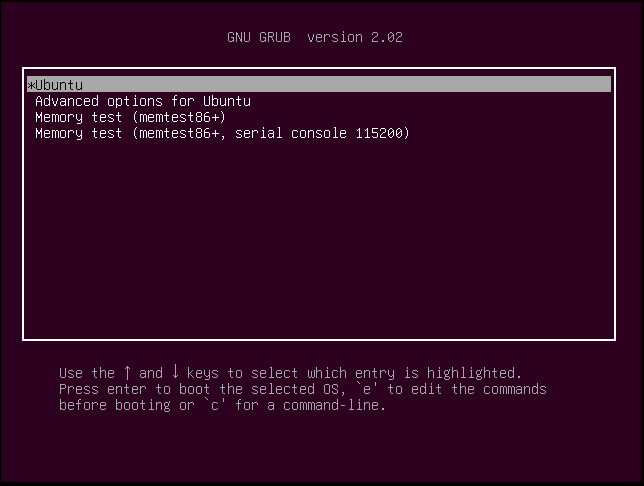
\includegraphics[width=0.8\textwidth]{chapters/09-boot/img/boot-grub.png}
  \caption{Ecran de boot GRUB}
  \label{fig:boot:boot-grub}
\end{figure}

În acest ecran observăm opțiunile de boot pentru GRUB. În mod tipic, un
utilizator selectează una dintre intrări și apoi apasă tasta \texttt{Enter} pentru a
boota folosind acea opțiune. În \labelindexref{Figura}{fig:boot:boot-grub} avem doar opțiuni de boot pentru Linux (Ubuntu). Pe un sistem de tip dual-boot, ecranul de boot GRUB va afișa intrări și pentru Windows.

Un utilizator poate alege să editeze o intrare GRUB. În acest caz utilizatorul
va apăsa tasta \texttt{e} și va accesa o nouă interfață ca în \labelindexref{Figura}{fig:boot:edit-grub}.
În interfața nouă putem modifica imaginea de kernel (de nucleu de sistem de operare)
folosită, putem modifica partiția rădăcină folosită sau opțiuni de boot pentru
kernel. O utilizare a editării opțiunilor de boot este recuperarea parolei
contului \texttt{root} folosind opțiunea \texttt{init=/bin/bash} așa cum am precizat în
\labelindexref{Secțiunea}{sec:user:linux-password-recovery}. Detalii despre
opțiunile de boot corespunzătoare nucleului sistemului de operare prezentăm în
\labelindexref{Secțiunea}{sec:boot:os}.

\begin{figure}[!htbp]
  \centering
  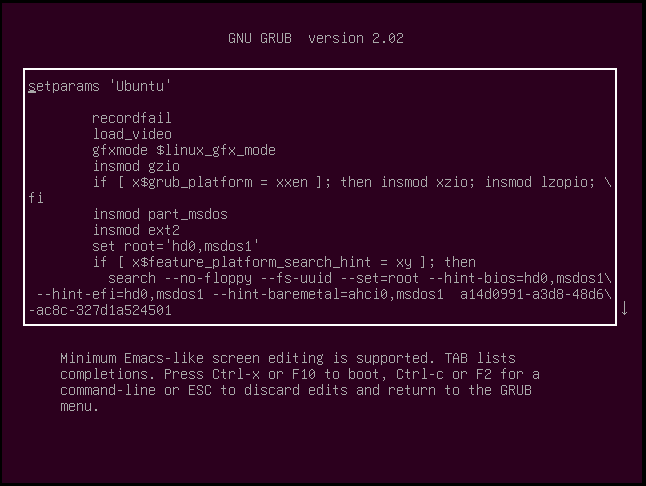
\includegraphics[width=0.8\textwidth]{chapters/09-boot/img/edit-grub.png}
  \caption{Editarea unei intrări în GRUB}
  \label{fig:boot:edit-grub}
\end{figure}

Opțiunile afișate de GRUB sunt încărcate din fișierul \file{/boot/grub/grub.cfg},
fișierul de configurare GRUB. Acest fișier nu se recomandă să fie editat manual;
fișierul este generat de comanda \cmd{update-grub} din analiza automată a sistemului și a configurărilor.
Comanda \cmd{update-grub} consultă
partițiile sistemului, detectează sisteme de operare și imagini de kernel,
consultă configurările din sistem și apoi generează fișierul
\file{/boot/grub/grub.cfg}.

Configurările GRUB, care devin persistente după rularea comenzii \cmd{update-grub}, se
realizează în fișierul \file{/etc/default/grub} și în fișierele din \file{/etc/grub.d/}. În
fișierul \file{/etc/default/grub} sunt variabile GRUB care afectează comportamentul
acestuia. \labelindexref{Listing}{lst:boot:grub-cfg} din fișierul \file{/etc/default/grub}.

\begin{screen}[caption={Configurare GRUB: /etc/default/grub},label={lst:boot:grub-cfg}]
student@uso:~$ cat /etc/default/grub
# If you change this file, run 'update-grub' afterwards to update
# /boot/grub/grub.cfg.
# For full documentation of the options in this file, see:
#  info -f grub -n 'Simple configuration'

GRUB_DEFAULT=0
GRUB_TIMEOUT_STYLE=hidden
GRUB_TIMEOUT=10
GRUB_DISTRIBUTOR=`lsb_release -i -s 2> /dev/null || echo Debian`
GRUB_CMDLINE_LINUX_DEFAULT="quiet splash"
GRUB_CMDLINE_LINUX=""
\end{screen}

Observăm la începutul fișierului comentariul care spune că aceste configurări
sunt apoi marcate persistente în fișierul de configurare \file{/boot/grub/grub.cfg}
după rularea comenzii \cmd{update-grub}. Opțiunile de mai sus reprezintă:

\begin{itemize}
  \item \texttt{GRUB\_DEFAULT}: indexul opțiunii implicite de boot a GRUB; în
		ecranul afișat către utilizator la bootare, dacă utilizatorul nu
		alege o opțiune, opțiunea implicită va fi aleasă
  \item \texttt{GRUB\_TIMEOUT}: după cât timp de la afișarea ecranului GRUB, timp în
		care utilizatorul nu a atins nici o tastă, se bootează în
                opțiunea implicită; valoarea \texttt{-1} înseamnă așteptare infinită până la alegerea explicită a unei opțiuni
  \item \texttt{GRUB\_TIMEOUT\_STYLE}: precizează cum va fi afișat ecranul de boot
    până la expirarea timpului de afișare; valoarea \texttt{hidden}
		înseamnă că nu se afișează nici un ecran, și după 10 secunde se
		bootează opțiunea implicită; în acel interval de 10 secunde
                utilizatorul poate apăsa tasta \texttt{Esc} pentru a cauza afișarea
		ecranului de boot
  \item \texttt{GRUB\_TIMEOUT\_LINUX\_DEFAULT}: adaugă opțiunile respective nucleului
		când bootează
\end{itemize}

În directorul \file{/etc/grub.d/} sunt fișiere de configurare pentru opțiuni GRUB.
Multe fișiere sunt predefinite pentru configurări dedicate. Dacă dorim să facem
configurări personale vom completa fișierele \file{/etc/grub.d/40\_custom} sau
\file{/etc/grub.d/41\_custom}. Aceste fișiere sunt citite literal și adăugate la
sfârșitul fișierului \file{/boot/grub/grub.cfg}.

Pentru detalii despre configurarea GRUB consultați documentația, fie online\footnote{\url{https://www.gnu.org/software/grub/manual/grub/}}, fie accesând pagina \cmd{info}: \cmd{info grub "Configuration"}.

\section{Pornirea kernelului și drivere}
\label{sec:boot:os}

Rolul bootloaderului este de a permite utilizatorului să selecteze un sistem de
operare în care să booteze, să configureze opțiunile acelui sistem de operare și
apoi să booteze în sistemul de operare.

Bootloaderul va încărca un fișier numit \textbf{imagine de kernel}, care conține codul
și datele sistemului de operare, și apoi va transfera controlul către acesta. Imaginea de
kernel (sau imaginea de nucleu de sisteme de operare) este practic un executabil
care conține implementarea nucleului (kernelului), componenta critică în
funcționarea sistemului.

Nucleul realizează configurarea componentelor hardware ale sistemului, încarcă
driverele de dispozitiv (\textit{device drivere}), montează sistemul de fișiere rădăcină
și apoi pornește procesul \texttt{init}, primul proces al sistemului, care, la rândul său,
va porni alte procese. Un driver este un fișier ce conține codul
pentru utilizarea și configurarea unui dispozitiv hardware. După investigarea
hardware-ului sistemului, nucleul sistemului de operare identifică dispozitivele
hardware și apoi încarcă de pe disc device driverele.

\subsection{Kernelul și driverele în Linux}
\label{sec:boot:os-linux}

Într-o configurație tipică, fișierul reprezentând imaginea de kernel în Linux se
găsește în \file{/boot/vmlinuz-$<$versiune$>$}, unde \texttt{$<$versiune$>$} este versiunea de sistem de
operare. Un exemplu este \file{/boot/vmlinuz-4.15.0-29-generic}. Acest fișier este
configurat să fie încărcat de bootloader. Este încărcat în memorie și apoi
executat, transferându-se controlul sistemului de operare. O investigație în
linia de comandă ne oferă informații despre această imagine:

\begin{screen}
student@uso:~$ file /boot/vmlinuz-4.15.0-29-generic
/boot/vmlinuz-4.15.0-29-generic: Linux kernel x86 boot executable bzImage, version 4.15.0-29-generic (buildd@lgw01-amd64-057) #31-Ubuntu SMP Tue Jul 17 15:39:52 UTC 2018, RO-rootFS, swap_dev 0x7, Normal VGA
\end{screen}

În cazul de față avem o imagine de kernel comprimată folosind algoritmul bzip2,
de unde și precizarea \texttt{executable bzImage}; tot ca referință la faptul că este
comprimată este și folosirea literei \texttt{z} în numele fișierului
\texttt{vmlinuz-4.15.0-29-generic}. Imaginea este de tip self-extracting: după ce este
încărcată în memorie de bootloader, se transferă controlul imaginii care conține
o secvență inițială de cod ce decomprimă restul fișierului și apoi îl execută.

Driverele sunt localizate, în Linux, în directorul \file{/lib/modules/$<$version$>$/kernel}
unde \texttt{$<$version$>$} este versiunea de sistem de operare. Driverele
corespunzătoare imaginii \file{/boot/vmlinuz-4.15.0-29-generic} se găsesc în directorul
\file{/lib/modules/4.15.0-29-generic/kernel/}. De fapt, în acel director se
găsesc modulele de kernel, componente externe nucleului care pot fi încărcate în
cadrul acestuia pentru a-i extinde funcționalitatea. Numim modul de kernel orice program extern nucleului care extinde funcționalitatea acestuia. Numim drivere acele module de kernel al căror rol este de a permite
utilizarea și configurarea componentelor hardware.  În Linux, un modul de kernel / driver este un fișier cu extensia \texttt{.ko}:

\begin{screen}
student@uso:~$ file /lib/modules/4.15.0-29-generic/kernel/drivers/net/ethernet/intel/e1000/e1000.ko
/lib/modules/4.15.0-29-generic/kernel/drivers/net/ethernet/intel/e1000/e1000.ko: ELF 64-bit LSB relocatable, x86-64, version 1 (SYSV), BuildID[sha1]=c2bcba22a6d98cf9d4c3735248bc48674ead034b, not stripped
\end{screen}

Observăm că driverul \texttt{e1000}, pentru plăci de rețea Intel, se găsește în fișierul
\texttt{e1000.ko}, fișier de tipul ELF \abbrev{ELF}{Executable and Linking Format} (\textit{Executable
and Linking Format}), formatul clasic de executabil pe Linux.

Driverele sunt încărcate fie de kernel la pornirea sistemului, după
identificarea componentelor hardware, fie în timp real, de programe dedicate sau
de utilizator. În lucrul cu module sau drivere, utilizatorul poate realiza
următoarele operații:

\begin{itemize}
  \item listarea modulelor încărcate în nucleu, folosind utilitarul \cmd{lsmod}
  \item încărcarea unui modul de kernel nou, folosind utilitarul \cmd{insmod} sau
    utilitarul \cmd{modprobe}
  \item descărcarea unui modul de kernel existent, folosind utilitarul \cmd{rmmod}
    sau comanda \cmd{modprobe -r}
  \item afișarea de informații despre un modul de kernel folosind utilitarul \cmd{modinfo}
\end{itemize}

\labelindexref{Listing}{lst:boot:modules} jos avem exemple de comenzi de lucru cu module de kernel:

\begin{screen}[caption={Lucrul cu module de kernel în Linux},label={lst:boot:modules}]
student@uso:~$ sudo lsmod
Module                  Size  Used by
btrfs                1150976  0
zstd_compress         163840  1 btrfs
xor                    24576  1 btrfs
[...]
minix                  32768  0
ntfs                  102400  0
[...]

student@uso:~$ sudo modinfo e1000
filename:       /lib/modules/4.15.0-118-generic/kernel/drivers/net/ethernet/intel/e1000/e1000.ko
version:        7.3.21-k8-NAPI
license:        GPL
description:    Intel(R) PRO/1000 Network Driver
author:         Intel Corporation, <linux.nics@intel.com>
[...]

student@uso:~$ sudo rmmod minix

student@uso:~$ sudo modprobe minix

student@uso:~$ sudo modprobe -r ntfs

student@uso:~$ sudo insmod /lib/modules/4.15.0-118-generic/kernel/fs/ntfs/ntfs.ko
\end{screen}

Comanda \cmd{insmod} primește ca argumente calea completă către fișierul ce conține
modulul de kernel în vreme ce comanda modprobe primește numele modulului și apoi
îl caută în directorul \file{/lib/modules/$<$version$>$}.

Dacă dorim încărcate anumite versiuni de module de kernel la pornirea
sistemului, sau dacă dorim să împiedicăm încărcarea anumitor module
(\textit{blacklisting}) atunci vom realiza configurări în fișierul \file{/etc/modules} sau în
directorul \file{/etc/modprobe.d/}.

În directorul \file{/boot/} pe lângă imagini de kernel, apar fișiere numite
\file{initrd.img-$<$version$>$}. De exemplu fișierul \texttt{/boot/initrd.img-4.15.0-29-generic}.
Acest fișier este numit \textit{ram disk image} și conține o serie de drivere
necesare pentru pornirea nucleului. Atunci când nucleul pornește trebuie să
încarce informații de pe disc. Pentru a le accesa are însă nevoie de driverul de
disc și de driverul de sistem de fișiere. O soluție ar fi să fie adăugate în
imaginea de kernel; dar, dat fiind numărul mare de discuri și de sisteme de
fișiere, ar rezulta o imagine de kernel mult prea mare și cu multe drivere
inutile pe sistemul curent. Soluția este adăugarea acestor drivere într-o
imagine separată: \textit{ram disk image}.

Imaginea de ram disk este încărcată de bootloader, așa cum am văzut în ecranul
de configurare a opțiunii GRUB din \labelindexref{Figura}{fig:boot:edit-grub}. Când nucleul
bootează, are referință la această imagine în memorie și poate folosi driverul de
disc și de sistem de fișiere corespunzător pentru a putea folosi discul.

Imaginea de ram disk este generată la instalarea unei versiuni noi de kernel și
poate fi generată la nevoie cu ajutorul comenzii \cmd{mkinitramfs}. Nu vom detalia
aici această comandă, puteți urmări pagina sa de manual sau exemple pe Internet.

După cum spuneam mai sus, în ecranul de bootloader sau în cadrul opțiunii
\texttt{GRUB\_CMDLINE\_DEFAULT} putem preciza opțiuni pentru kernel care afectează modul în
care acesta bootează și rulează. Comanda echivalentă folosită pentru bootarea
kernelului, împreună cu opțiunile aferente, se găsește în fișierul
\file{/proc/cmdline}:

\begin{screen}
student@uso:~$ cat /proc/cmdline
BOOT_IMAGE=/boot/vmlinuz-4.15.0-34-generic root=UUID=a14d0991-a3d8-48d6-ac8c-327d1a524501 ro quiet splash
\end{screen}

Dintre opțiunile de boot ale nucleului, precizăm:

\begin{itemize}
  \item opțiunile \texttt{debug}, \texttt{verbose}, \texttt{quiet} care configurează nivelul de
		detaliu al mesajelor de boot afișate la pornirea kernelului
  \item opțiunea \texttt{splash} activează splashscreenul la pornirea sistemului,
		în loc să afișeze mesajele de boot
  \item opțiunea \texttt{noacpi} dezactivează ACPI \abbrev{ACPI}{Advanced
    Configuration and Power Interface} (\textit{Advanced Configuration and
                Power Interface}) o componentă PC care uneori este cauzatoare de
		probleme
\end{itemize}

O listă completă a acestor opțiuni găsiți în documentația nucleului\footnote{\url{https://www.kernel.org/doc/html/v5.9/admin-guide/kernel-parameters.html}}.

După ce sistemul de operare a pornit, putem afla informații despre acesta. Pe
lângă aflarea liniei de comandă echivalente din fișierul \file{/proc/cmdline}, mai
putem afla versiunea nucleului care rulează folosind \cmd{uname}:

\begin{screen}
student@uso:~$ uname -a
Linux uso 4.15.0-34-generic #37-Ubuntu SMP Mon Aug 27 15:21:48 UTC 2018 x86_64 x86_64 x86_64 GNU/Linux
\end{screen}

De asemenea, pentru depanare sau informare, nucleul transmite informații care se
jurnalizează. Pentru accesarea jurnalului folosim comanda \cmd{dmesg}, ca mai jos:

\begin{screen}
student@uso:~$ dmesg
[   0.000000] Linux version 4.15.0-34-generic (buildd@lgw01-amd64-047) (gcc version 7.3.0 (Ubuntu 7.3.0-16ubuntu3)) #37-Ubuntu SMP Mon Aug 27 15:21:48 UTC 2018 (Ubuntu 4.15.0-34.37-generic 4.15.18)
[   0.000000] Command line: BOOT_IMAGE=/boot/vmlinuz-4.15.0-34-generic root=UUID=a14d0991-a3d8-48d6-ac8c-327d1a524501 ro quiet splash
[   0.000000] KERNEL supported cpus:
[   0.000000]   Intel GenuineIntel
[   0.000000]   AMD AuthenticAMD
[...]
\end{screen}

\section{Pornirea init și a serviciilor de startup în Linux}
\label{sec:boot:init-linux}

După ce nucleul și driverele sunt încărcate și sistemul de operare este
inițializat, trebuie pornite primele procese. Pentru început se pornește primul
proces, numit generic \textbf{init}, care apoi pornește alte procese. Așa cum am precizat în
\labelindexref{Secțiunea}{sec:process:linux-hierarchy}, procesul init este în vârful
ierarhiei proceselor având ca roluri crearea primelor procese din sistemul de
operare și adoptarea proceselor orfane.

În mod tradițional, init era procesul pornit din executabilul \file{/sbin/init} și se
numea System V init, după numele unei versiuni importante de UNIX (UNIX System
V). În mod curent implementarea cea mai răspândită de init este \textbf{systemd}, cu
executabilul aflat în \file{/lib/systemd/systemd}:

\begin{screen}
student@uso:~$ ls -l /sbin/init
lrwxrwxrwx 1 root root 20 aug  6 17:34 /sbin/init -> /lib/systemd/systemd
\end{screen}

Observăm că \file{/sbin/init} este, pe sistemele Linux moderne, un fișier de tipul
legătură simbolică la fișierul \file{/lib/systemd/systemd}. Astfel că, pe sistemele
moderne, configurarea init echivalează configurării systemd.

Procesul principal systemd rulează ca procesul cu PID-ul 1. Există posibilitatea
creării unui proces per utilizator prin transmiterea opțiunii \texttt{-{}-user} comenzii
\texttt{systemd}. Acest lucru este util atunci când dorim să creăm și să gestionăm
servicii la nivelul utilizatorului, la la nivelul sistemului.

Serviciile sunt procese dedicate, de obicei procese daemon (revedeți \labelindexref{Secțiunea}{sec:process:daemon}), care oferă
funcționalități suplimentare sistemului sau care gestionează buna funcționare a
acestuia. Serviciile sunt în general pornite și gestionate de systemd.

În mod tradițional, în implementarea veche (System V) de init, serviciile se
configurau și rulau cu ajutorul scripturilor de inițializare din directorul \file{/etc/init.d/}.
Pentru a menține compatibilitatea, systemd folosește în continuare acele
scripturi de inițializare, pe care le le putem localiza pe sistemele moderne:

\begin{screen}
student@uso:~$ ls /etc/init.d/
acpid      apport            cron          dns-clean      [...]
alsa-utils avahi-daemon      cups          gdm3           [...]
anacron    bluetooth         cups-browsed  grub-common    [...]
apparmor   console-setup.sh  dbus          hddtemp        [...]
\end{screen}

În systemd, serviciile, împreună cu alte componente, sunt numite \texttt{units}. Pentru a
vizualiza toate unitățile systemd, folosim comanda \cmd{systemd -{}-list-units}:

\begin{screen}
student@uso:~$ systemctl list-units | head -100
UNIT                     LOAD   ACTIVE SUB       DESCRIPTION
proc-sys-fs-[...]        loaded active waiting   Arbitrary Executable File Formats File System Automount Point
sys-devices-[...]        loaded active plugged   VBOX_CD-ROM
sys-devices-[...]        loaded active plugged   82540EM Gigabit Ethernet Controller (PRO/1000 MT Desktop Adapter)
sys-devices-[...]        loaded active plugged   82801AA AC'97 Audio Controller
sys-devices-[...]        loaded active plugged   82540EM Gigabit Ethernet Controller (PRO/1000 MT Desktop Adapter)
sys-devices-[...]        loaded active plugged   VBOX_HARDDISK 1
sys-devices-[...]        loaded active plugged   VBOX_HARDDISK
sys-devices-[...]        loaded active plugged   VBOX_HARDDISK 1
\end{screen}

Dacă dorim să afișăm informații, oprim, porni sau reporni servicii, putem folosi
fie interfața clasică \file{/etc/init.d/}, fie comanda \cmd{service}, fie comanda \cmd{systemctl}.
Mai jos sunt comenzile în toate formele pentru afișarea stării serviciului SSH (pentru conexiune
la distanță) și pentru pornirea serviciului:

\begin{screen}
student@uso:~$ /etc/init.d/ssh status
student@uso:~$ service ssh status
student@uso:~$ systemctl status ssh.service
student@uso:~$ sudo /etc/init.d/ssh start
student@uso:~$ sudo service ssh start
student@uso:~$ sudo systemctl start ssh.service
\end{screen}

Dacă dorim să oprim sau să repornim serviciul, folosim parametrul \texttt{stop},
respectiv \texttt{restart}, în loc de \texttt{start}.

Dacă dorim adăugarea de servicii în sistem putem să le adăugăm în configurarea
\cmd{systemd} sau putem folosi \cmd{supervisor}. Vom detalia în
\labelindexref{Secțiunea}{sec:auto-infosys-services}

\subsection{Pornirea terminalelor de login}
\label{sec:boot:init-linux:login}

Ulterior pornirii serviciilor inițiale (\textit{startup processes}), init/systemd trebuie să
pornească și terminalele de login, numite terminal virtuale, unde utilizatorul
se va putea autentifica. Pe sistemele cu interfață grafică aceste terminale
virtuale nu sunt accesibile direct pentru că este pornit mediul grafic. Pentru
accesarea lor, se folosesc combinațiile de taste \texttt{Ctrl+Alt+F1}, \texttt{Ctrl+Alt+F2}, \ldots,
\texttt{Ctrl+Alt+F6}. Pe un sistem fără interfață grafică se
vede implicit primul terminal putându-se accesa celelalte terminale folosind
combinațiile de taste \texttt{Ctrl+Alt+F2}, \ldots, \texttt{Ctrl+Alt+F6}.

Mediul grafic, în cazul în care este prezent, poate porni în locul unui terminal
virtual. Acesta va fi accesibil de obicei prin \texttt{Ctrl+Alt+F1} sau \texttt{Ctrl+Alt+F7}, dar
orice configurație este posibilă.

Terminalele virtuale sunt pornite și gestionate de init/systemd prin următorul flux, prezentat în \labelindexref{Figura}{fig:boot:login}.

\begin{enumerate}
  \item systemd pornește procese numite \cmd{getty} care reprezintă interfața de
		comunicare cu terminalul virtual.
  \item \cmd{getty} afișează un prompt de utilizator unde se introduce
		numele de utilizator și parola.
  \item \cmd{getty} pornește procesul \cmd{login} care citește parola
          utilizatorului și o verifică în fișierul \file{/etc/shadow}
        \item dacă parola este corectă, procesul \cmd{login} pornește shellul descris ca
          ultima coloana din linia corespunzătoare utilizatorului în fișierul \file{/etc/passwd}
\end{enumerate}

\begin{figure}[htbp]
	\centering
	\def\svgwidth{\columnwidth}
	\includesvg{chapters/09-boot/img/systemd-login.svg}
	\caption{Pornirea terminalelor virtuale și a shellurilor}
        \label{fig:boot:login}
\end{figure}

Putem vizualiza unitățile gestionate de systemd pentru terminalele virtuale folosind comanda de mai jos:

\begin{screen}
student@uso:~$ systemctl list-units | grep getty
getty@tty2.service           loaded active running   Getty on tty2
getty@tty3.service           loaded active running   Getty on tty3
getty@tty4.service           loaded active running   Getty on tty4
getty@tty5.service           loaded active running   Getty on tty5
getty@tty6.service           loaded active running   Getty on tty6
system-getty.slice           loaded active active    system-getty.slice
getty.target                 loaded active active    Login Prompts
\end{screen}

Observăm în cadrul comenzii că sunt cinci terminale virtuale, de la \texttt{tty2} până la
\texttt{tty6}. Putem observa și procesele aferente celor cinci terminale virtuale, gestionate
de procesul \cmd{agetty}, o implementare de \cmd{getty}.

\begin{screen}
student@uso:~$ ps -f -C agetty
UID       PID  PPID  C STIME TTY          TIME CMD
root     4453     1  0 14:27 tty2     00:00:00 /sbin/agetty [...]
root     4454     1  0 14:27 tty3     00:00:00 /sbin/agetty [...]
root     4455     1  0 14:27 tty4     00:00:00 /sbin/agetty [...]
root     4456     1  0 14:27 tty5     00:00:00 /sbin/agetty [...]
root     4457     1  0 14:27 tty6     00:00:00 /sbin/agetty [...]
\end{screen}

După o autentificare corectă la un terminal virtual este pornit shellul.
Shellul poate fi pornit și dintr-un emulator de terminal din interfața grafică
și dintr-un pseudo-terminal creat printr-o conexiune SSH. În toate situațiile
shellul folosește niște fișiere de configurare specifice care personalizează
experiența utilizatorului în linia de comandă, așa cum am prezentat în \labelindexref{Secțiunea}{sec:cli:shell-start:config}.

\section{Anexă: Resetarea parolei administrative}
\label{sec:boot:pass-reset}

Este posibil ca pentru un sistem să pierdem parola administrativă, a contului
root sau a contului Administrator și să fie nevoie de resetarea acesteia. În
\labelindexref{Secțiunea}{sec:user:linux-password-recovery} și \labelindexref{Secțiunea}{sec:user:windows-password-recovery} am precizat modurile
uzuale de resetare a parolei administrative și în Linux și în Windows. În Linux
folosim opțiunea \texttt{init=/bin/bash} la bootarea sistemului de operare, editând
intrarea în bootloader, sau folosim unui USB stick bootabil sau CD-ROM. În
Windows folosim Ultimate Boot CD.

În Linux este posibil să configurăm parolă de acces la bootloader (GRUB) și
atunci opțiunea cu editarea intrării în bootloader nu funcționează. Rămâne însă
o opțiune folosirea unui USB stick bootabil care nu necesită editarea
opțiunilor.

Chiar și așa, este posibil să fie dezactivat din firmware-ul de boot folosirea
USB sau CD-ROM pentru bootare. Sau să fie configurată parolă de acces la firmware
care nu permite editarea opțiunilor și, deci, adăugarea opțiunii de boot USB sau
CD-ROM. Pentru aceasta avem soluția desfacerii unității fizice a sistemului și extragerea bateriei
CMOS care va duce la resetarea configurării firmware-ului de boot la o valoare
implicită, fără parolă. Ulterior vom activa bootarea de pe USB sau CD-ROM și vom
reseta parola administrativă folosind un USB stick sau CD-ROM bootabil. Evident,
resetarea parolei firmware-ului de boot prin extragerea bateriei CMOS necesită
acces fizic la sistem.

O formă mai directă de a trece de parola de firmware de boot sau cea de
bootloader este detașarea discului din unitate și atașarea acestuia la o altă
unitate. Apoi se bootează acel sistem cu un stick USB sau CD-ROM bootabil și se
resetează parola. Pentru a preveni acest lucru o soluție este criptarea
discului, lucru ce face imposibilă orice modificare fără accesul la parolă.

\section{Anexă: Crearea unui stick USB bootabil cu Linux}
\label{sec:boot:usb-linux}

Pentru a instala un sistem de operare Linux pe un PC, avem nevoie de un mediu de
boot. În mod obișnuit, acest mediu va fi un stick USB bootabil. Pentru început
acest stick trebuie să fie partiționat și apoi marcată partiția principală ca
fiind bootabilă. Pașii de pregătire ai mediului de boot sunt:

\begin{enumerate}
	\item Ștergerea vechilor componentele de pe stickul USB. Presupunând că
          stickul USB este accesibil prin intrarea \file{/dev/sdb}, rulăm
		comanda

\begin{screen}
dd if=/dev/zero of=/dev/sdb bs=1M count=16
\end{screen}

    Adică scriem \texttt{16MB} de zero-uri anulând tabela de partiții și pregătind discul.

	\item Crearea tabelei de partiții și apoi unei partiții FAT32 și
		marcarea acesteia ca fiind bootabilă. Pentru aceasta folosim
                utilitarul \cmd{gparted} (cu interfața grafică), accesând opțiunile:
                \begin{enumerate}
                  \item \texttt{Device} $\rightarrow$ \texttt{Create Partition Table}
                  \item click dreapta pe spațiu $\rightarrow$ \texttt{New}
                  \item click dreapta pe partiție $\rightarrow$ \texttt{Manage Flags} $\rightarrow$ \texttt{boot}
                \end{enumerate}

\end{enumerate}

În acest moment avem un stick USB cu o partiție FAT32 bootabilă.

Pentru scrierea de informații pe stickul USB, descărcăm un fișier \texttt{.iso}
cu distribuția
Linux dorită. Apoi folosim utilitarul \cmd{unetbootin} (pe orice
platformă)\footnote{\url{https://unetbootin.github.io}}, cu interfață grafică.
Înainte de folosirea sa, trebuie să fie montat stickul USB, fie automat fie
printr-o comandă de forma:

\begin{screen}
student@uso:~$ sudo mkdir /mnt/sdb1
student@uso:~$ sudo mount /dev/sdb1 /mnt/sdb1
\end{screen}

În interfața \cmd{unetbootin} selectăm fișierul \texttt{.iso} pe care dorim să îl scriem și
destinația unde este montat stickul, adică \file{/mnt/sdb1} în cazul nostru.

O alternativă, care permite crearea unui stick USB cu Linux folosind Windows,
este folosirea utilitarului Rufus\footnote{\url{https://rufus.akeo.ie}} urmărind
indicațiile de
aici\footnote{\url{https://tutorials.ubuntu.com/tutorial/tutorial-create-a-usb-stick-on-windows}}.

\section{Anexă: Crearea unui stick USB bootabil cu Windows}
\label{sec:boot:usb-windows}

Pentru crearea unui stick bootabil cu Windows, pregătim mediul de instalare
(stickul USB) în mod similar cu instalarea Linux, cu o diferență: partiția
trebuie să fie formatată NTFS.

Apoi se urmează pașii de mai jos, detaliați și
aici\footnote{\url{https://askubuntu.com/a/487970}}:

\begin{enumerate}
  \item Se montează fișierul \texttt{.iso} cu imaginea de Windows.

\begin{screen}
student@uso:~$ mkdir iso-mnt/
student@uso:~$ sudo mount -o loop windows.iso iso-mnt/
\end{screen}

	\item Se montează stickul USB:

\begin{screen}
student@uso:~$ sudo mkdir /mnt/sdb1
student@uso:~$ sudo mount /dev/sdb1 /mnt/sdb1
\end{screen}

	\item Se copiază tot conținutul din imaginea de Windows pe stickul
		USB:

\begin{screen}
student@uso:~$ sudo cp -r iso-mnt/* /mnt/sdb1/
\end{screen}

	\item Se instalează GRUB pe stickul USB:

\begin{screen}
sudo grub-install --target=i386-pc --boot-directory="/mnt/sdb1/boot" /dev/sdb
\end{screen}

        \item Se generează fișierul \file{/mnt/sdb1/boot/grub/grub.cfg} cu următorul
		conținut:

\begin{screen}
echo "If you see this, you have successfully booted from USB :)"
insmod ntfs
insmod search_fs_uuid
search --no-floppy --fs-uuid <UUID> --set root
ntldr /bootmgr
boot
\end{screen}

    iar în loc de \texttt{$<$UUID$>$} scriem identificatorul pe care îl obținem folosind comanda:

\begin{screen}
student@uso:~$ sudo blkid /dev/sdb1
\end{screen}
        \item Demontăm stickul USB și fișierul \texttt{.iso}:

\begin{screen}
student@uso:~$ sudo umount /mnt/sdb1
student@uso:~$ sudo umount iso-mnt/
\end{screen}

\end{enumerate}

Acum putem folosi stickul pentru a boota Windows.

\section{Anexă: Adăugarea unei intrări GRUB pentru UDPCast}
\label{sec:boot:updcast}

Pentru a demonstra o configurare particulară pentru GRUB, vom descrie instalarea
UDPcast pe disc. Va putea fi bootat de pe disc prin GRUB.
UDPCast\footnote{\url{http://www.udpcast.linux.lu}} este o imagine bootabilă de
CD care permite transferul prin rețea al unui disc de la o sursă către mai multe
destinații, asigurând astfel o clonare a discului.

Pentru a adăuga o intrare în GRUB pentru UDPCast și pentru a boota astfel în
GRUB fără a fi nevoie de un stick USB sau un CD-ROM bootabil, urmăm pașii:

\begin{enumerate}
  \item Obținem fișierul \texttt{.iso} UDPCast:

\begin{screen}
student@uso:~$ wget http://www.udpcast.linux.lu/20120424/udpcd.iso
\end{screen}

        \item Montăm fișierul \texttt{.iso}:

\begin{screen}
student@uso:~$ mkdir iso-mnt/
student@uso:~$ sudo mount -o loop udpcd.iso iso-mnt/
student@uso:~$ ls iso-mnt/
ISOLINUX.BIN  ISOLINUX.CFG boot.catalog  initrd  linux pxelinux.0
\end{screen}

    Din conținutul fișierului \texttt{.iso} ne interesează fișierele \texttt{initrd} și \texttt{linux}, adică
imaginea de ram disk și imaginea de kernel.

        \item Copiem imaginea de ram disk si cea de kernel într-un director din \file{/boot}:

\begin{screen}
student@uso:~$ sudo mkdir /boot/udpcast
student@uso:~$ sudo cp iso-mnt/{initrd,linux} /boot/udpcast
student@uso:~$ ls /boot/udpcast
initrd linux
\end{screen}

        \item Adăugăm configurarea corespunzătoare în fișierul \file{/etc/grub.d/40\_custom}

\begin{screen}
student@uso:~$ sudo blkid /dev/sda1
/dev/sda1: UUID="a14d0991-a3d8-48d6-ac8c-327d1a524501" TYPE="ext4" PARTUUID="df4f561b-01"
student@uso:~$ sudo vi /etc/grub.d/40_custom
student@uso:~$ cat /etc/grub.d/40_custom
#!/bin/sh
exec tail -n +3 $0
# This file provides an easy way to add custom menu entries.  Simply type the
# menu entries you want to add after this comment.  Be careful not to change
# the 'exec tail' line above.

menuentry 'UDPCast' {
       insmod part_msdos
       insmod ext2
       set root='(hd0,msdos1)'
       search --no-floppy --fs-uuid --set=root a14d0991-a3d8-48d6-ac8c-327d1a524501
       linux   /boot/udpcast/linux root=01:00
       initrd  /boot/udpcast/initrd
}
\end{screen}

    În configurarea GRUB am folosit UUID-ul partiției \file{/dev/sda1}, partiția unde se
    găsește directorul \file{/boot} (\texttt{a14d0991-a3d8-48d6-ac8c-327d1a524501})
pe care l-am descoperit cu ajutorul comenzii blkid. Am folosit
    construcția \texttt{(hd0,msdos1)} pentru a identifica prima partiție din
    primul hard disk, adică \file{/dev/sda1}.

	\item Actualizăm configurația GRUB:

\begin{screen}
student@uso:~$ sudo update-grub
Generating grub configuration file ...
[...]
done
student@uso:~$ grep UDPCast /boot/grub/grub.cfg
menuentry 'UDPCast' {
\end{screen}

În ultima comandă am verificat că intrarea a fost adăugată în fișierul de configurare GRUB: \file{/boot/grub/grub.cfg}.

        \item Demontăm fișierul \texttt{.iso}:

\begin{screen}
student@uso:~$ sudo umount iso-mnt
student@uso:~$ sudo rmdir iso-mnt
\end{screen}

	\item Repornim sistemul și apoi vom avea în GRUB intrarea aferentă UDPCast.
\end{enumerate}

\section{Anexă: Booting în Windows}
\label{sec:boot-init-win}

În Windows 7, 8 și 10, bootarea se bazează pe trei componente:

\begin{itemize}
  \item Windows Boot Manager (\file{Bootmgr.exe})
  \item bootloaderul sistemului de operare (\file{Windload.exe})
  \item loaderul unui sistem suspendat (\file{Winresume.exe})
\end{itemize}

A treia componentă este folosită doar pentru încărcarea unui sistem de operare suspendat/hibernat.

Windows Boot Manager este o componentă generică ce permite selectarea între mai
multe instanțe de sistem de operare Windows de pe un sistem dat. Windows Boot
Manager prezintă utilizatorului opțiunile de sistem de operare pe care să
booteze; după ce utilizatorul alege opțiunea respectivă, Windows Boot Manager
încarcă bootloaderul aferent și acesta, ulterior, va încărca sistemul de
operare.

Opțiunile de boot, însemnând ce sisteme de operare sunt disponibile și ce
opțiuni de boot sunt folosite pentru un sistem de operare, sunt reținute într-o
zonă numită BCD \abbrev{BCD}{Boot Configuration Data} (\textit{Boot Configuration Data}),
zonă ce poate fi editată folosind \cmd{BCDEdit.exe}, un utilitar inclus în Windows.

Detalii despre procesul de boot în Windows găsiți în
documentație\footnote{\url{https://docs.microsoft.com/en-us/windows-hardware/drivers/devtest/introduction-to-boot-options}}.

\section{Concluzii}
\label{sec:boot:conclusion}

Un sistem de calcul parcurge mai mulți pași din momentul pornirii acestuia
(apăsării pe butonul de \textit{power-on}) până la pornirea primelor procese interactive,
în general shellul.

Un utilizator are nevoie să știe procesul de boot pentru a putea depana probleme
ce pot apărea, pentru a configura componentele pornite și opțiunile acestora.

În general un sistem de calcul dispune de un firmware de boot, încărcat în
memorie și rulat imediat după pornirea sistemului. Acesta încarcă și transferă
controlul unui bootloader care încarcă și transferă controlul sistemului de
operare. Sistemul de operare configurează hardware-ul și pornește primele
procese din sistem. Procesul de boot se consideră încheiat când utilizatorul are acces la sistem, prin intermediul unui shell (CLI sau GUI).

Conceptual pașii sunt similari, dar la nivel practic apar diferențe între
tipurile de sisteme de calcul și sisteme de operare.
